\documentclass[12pt]{article} % use larger type; default would be 10pt
\usepackage[utf8]{inputenc} % set input encoding (not needed with XeLaTeX)

%%% PAGE DIMENSIONS
\usepackage{geometry} % to change the page dimensions
\geometry{a4paper} % or letterpaper (US) or a5paper or....
\geometry{margin=2cm} % or letterpaper (US) or a5paper or....

\usepackage{graphicx} % support the \includegraphics command and options
\usepackage[parfill]{parskip} % Activate to begin paragraphs with an empty line rather than an indent
\usepackage{times} % for Times Roman default font

%%% PACKAGES
\usepackage{booktabs} % for much better looking tables
\usepackage{array} % for better arrays (eg matrices) in maths
\usepackage{paralist} % very flexible & customisable lists (eg. enumerate/itemize, etc.)
\usepackage{verbatim} % adds environment for commenting out blocks of text & for better verbatim
\usepackage{subfig} % make it possible to include more than one captioned figure/table in a single float

%%% HEADERS & FOOTERS
\usepackage{fancyhdr} % This should be set AFTER setting up the page geometry
\pagestyle{fancy} % options: empty , plain , fancy
\renewcommand{\headrulewidth}{0pt} % customise the layout...
\lhead{}\chead{}\rhead{}
\lfoot{}\cfoot{\thepage}\rfoot{}

\makeatletter
\renewcommand{\maketitle}{%
  {\bfseries{\scshape{\Large{\@title\par}}}}
}
\makeatother

\hyphenation{Kiwi-bank} % otherwise it may get hyphenated as Ki-wibank

%%% END Article customizations

%%% The "real" document content comes below...

\title{Sylvia Tops Route: 30-31 January 2018}

\begin{document}
  \maketitle
This was really a recce, undertaken to investigate the route up to the Sylvia Tops from the Nina Hut track.  Apparently this route is maintained by NZDA, and we wanted to check it out before undertaking the entire circuit via Devil-skin Saddle.

The route is sign-posted off to the left about 35-40 minutes from the road.  It was probably a bit quicker this time as it has been so dry that we didn't have to be nimble through bog-holes.  We pitched the tent at the river, a further 10 minutes or so from the turn-off.  We'd had dinner before leaving, so it only remained to have a dip in the pool before turning in (and doing some crossword puzzles).

The following day we crossed the river near the top of the rapids as the water level was low and this was more-or-less opposite the large orange triangle marking the start of the track.  The track was not as well cut or marked as the Mt Norma Route but was nevertheless relatively easy to follow with a bit of care.  However, since most of the marking was done using pink flagging tape this could change quickly as the tape comes off.  The river is at about 620m and the bush line at about 1300m, and this climb took about an hour and a half.  There's a tall white pole just beyond the bush edge.  From here we climbed almost to high-point 1624, initially heading due west to get on the ridge leading to this high-point.  It was very windy on the ridge, and after a quick look at the route to Devil-skin Saddle (doable but a sharper ridge than I had expected), I scuttled back down to meet Robyn.  From the high-point the true bearing is 80$^o$ (i.e., current magnetic 58$^o$) to the white pole.

\begin{figure}[ht]
%\centering
\begin{minipage}{.5\linewidth}
\begin{flushleft}
   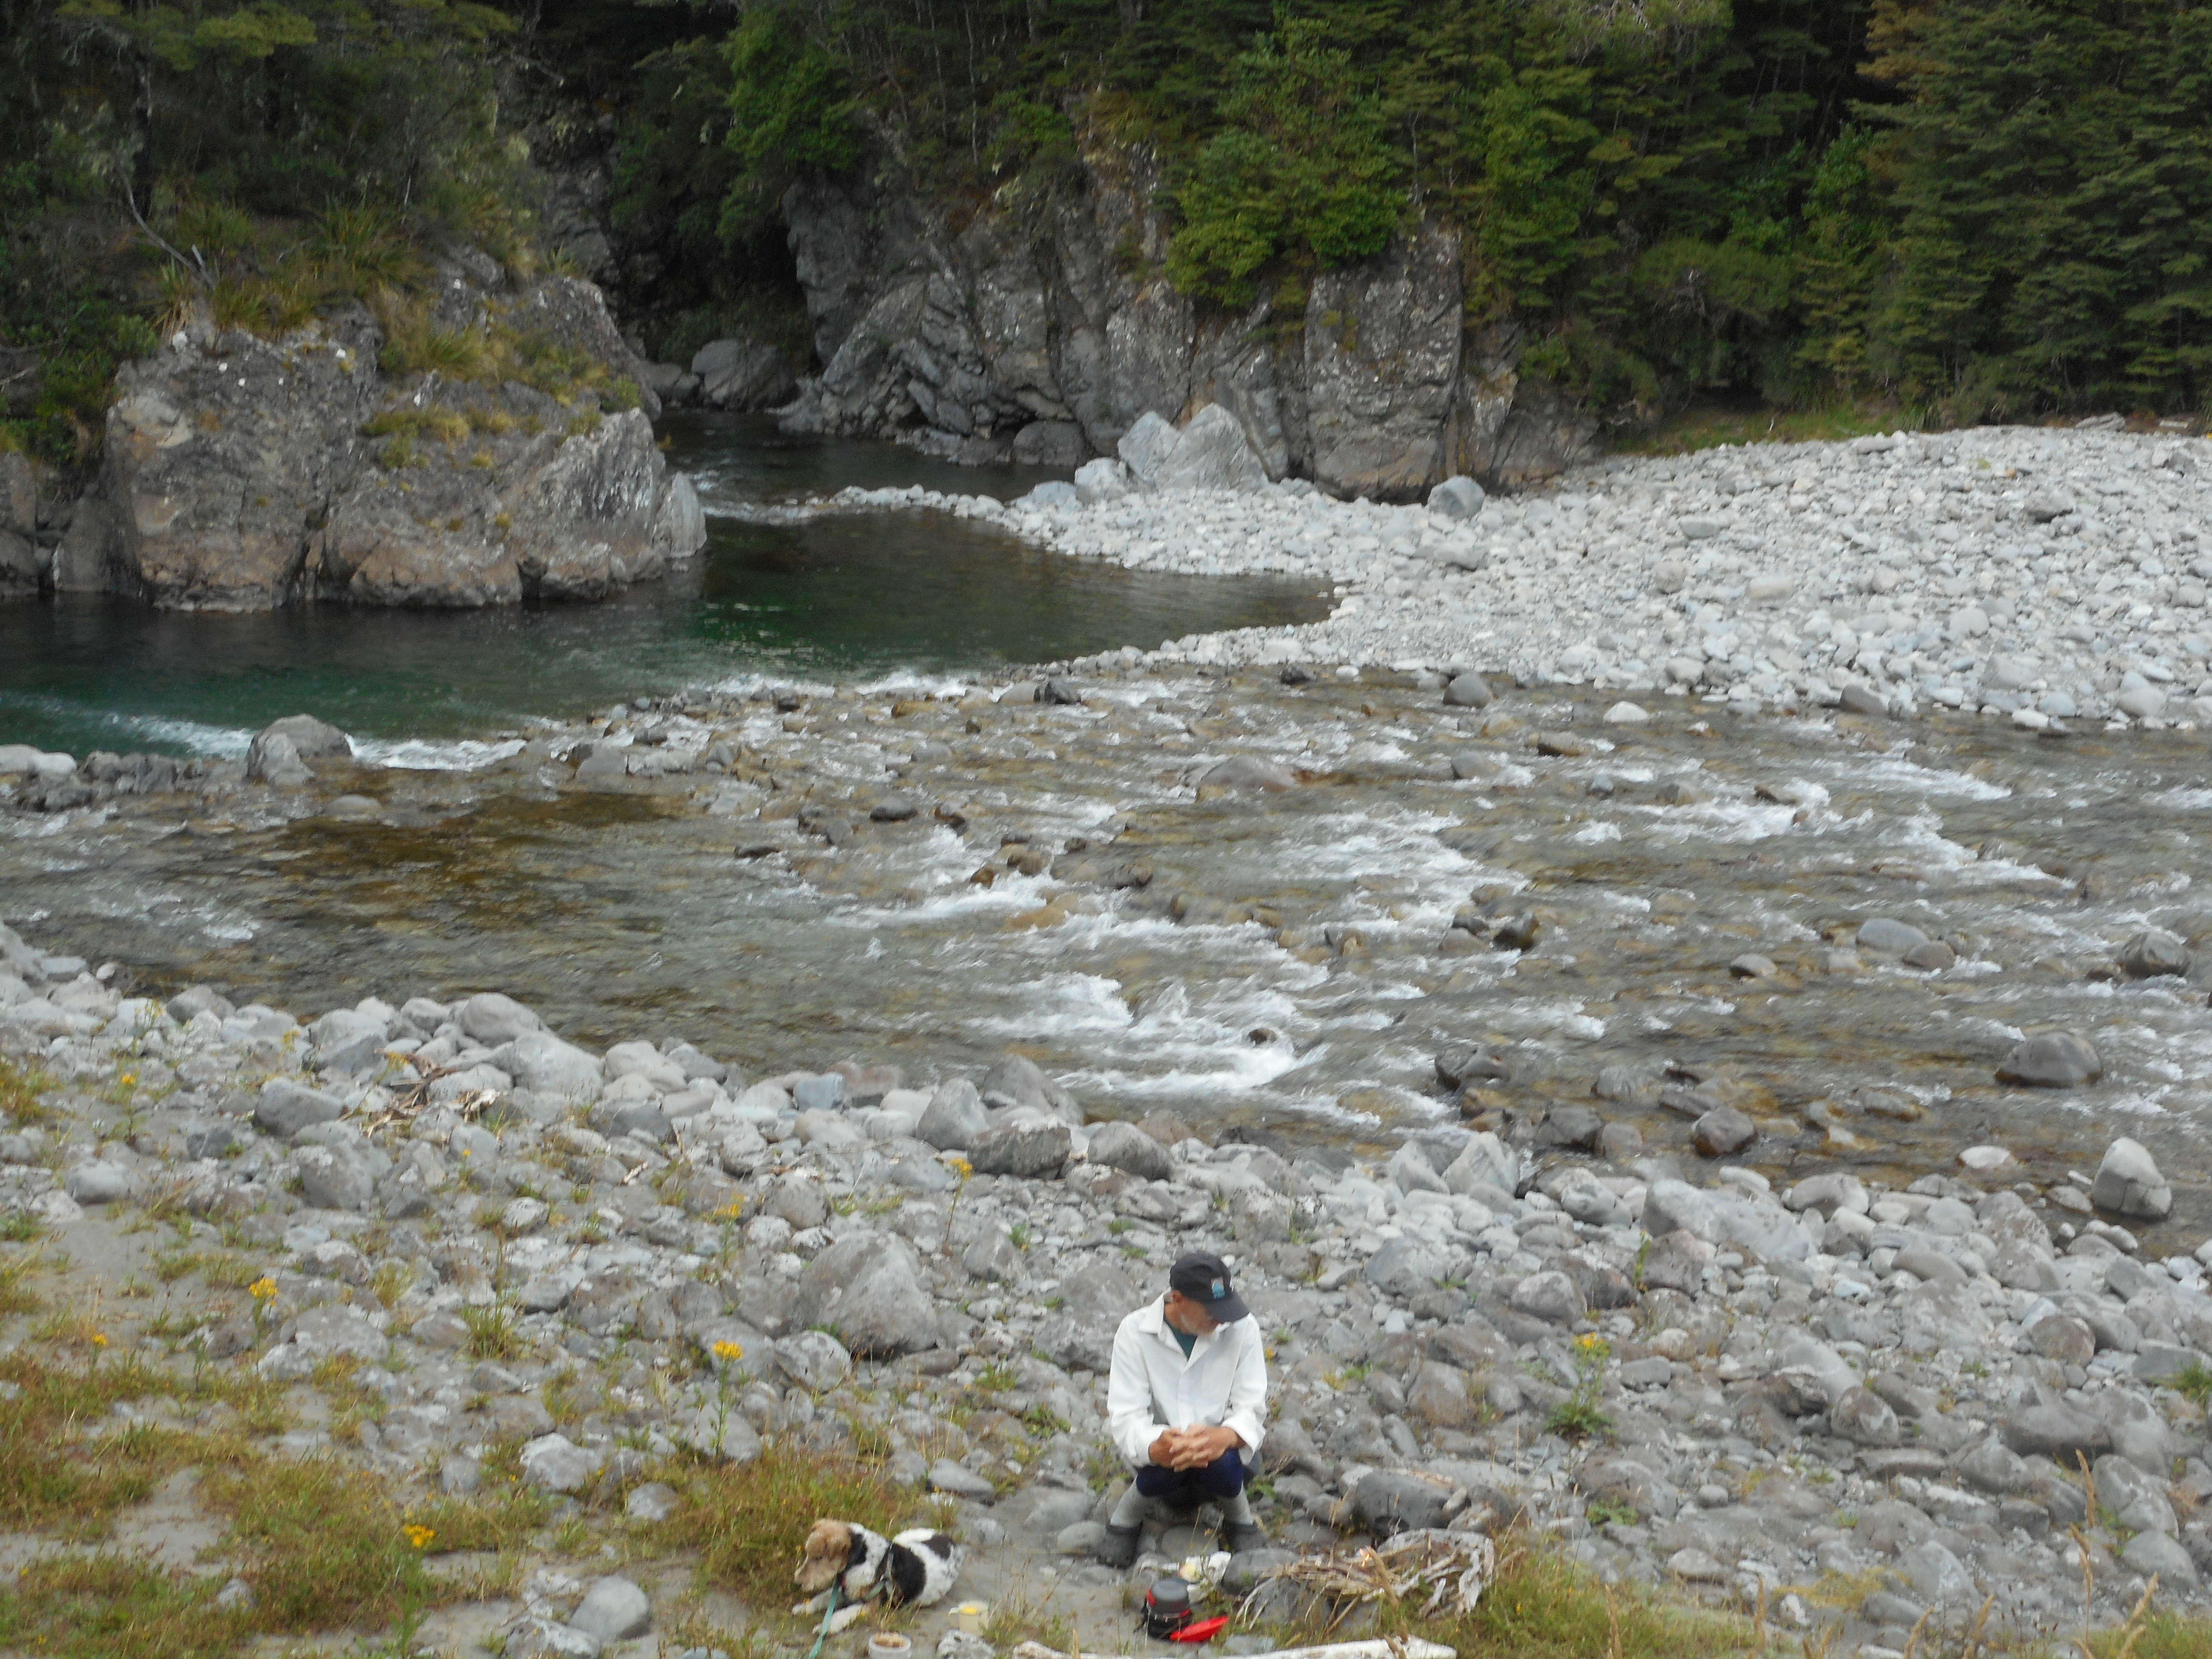
\includegraphics[width=8cm]{SylviaTopsRoute30January2018Photo1}
\end{flushleft}
\end{minipage}
\begin{minipage}{.5\linewidth}
\begin{flushright}
    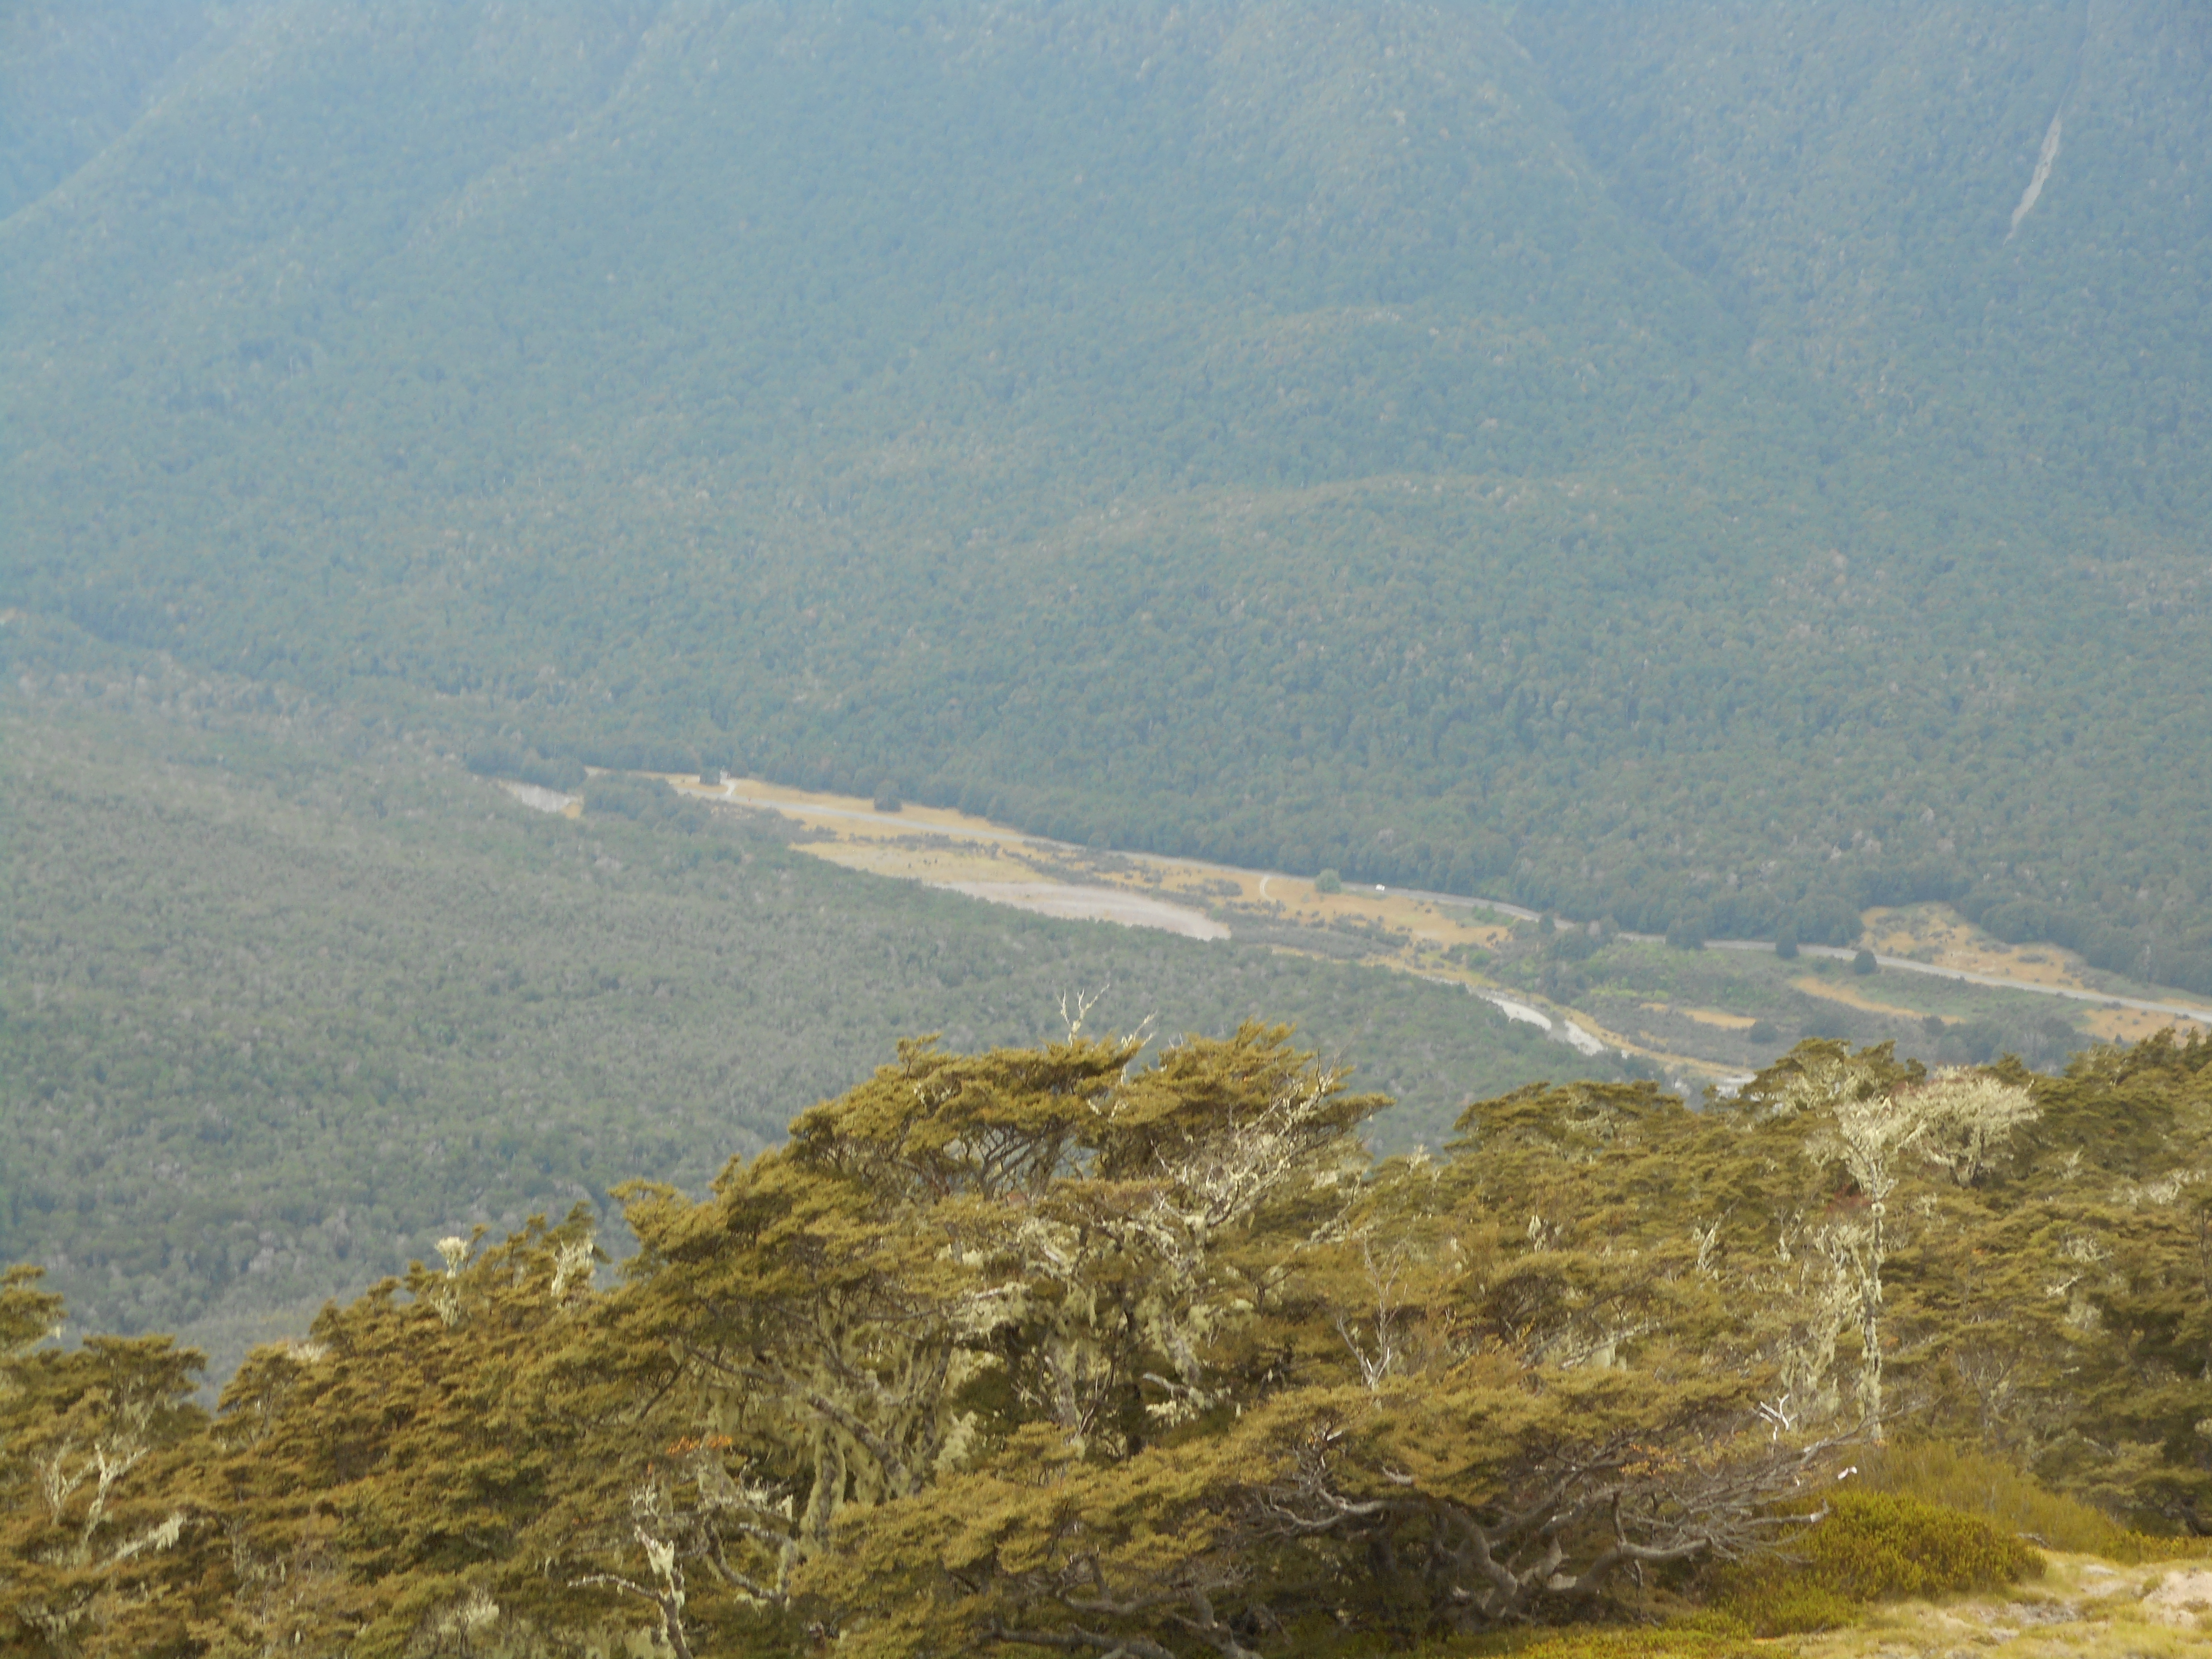
\includegraphics[width=8cm]{SylviaTopsRoute30January2018Photo2}
\end{flushright}
\end{minipage}
\end{figure}
 
The return walk was uneventful, other than the excessive number of sandflies at the tent site which made packing the tent a bit unpleasant.

\begin{flushright}
Robyn, Peter and dog
\end{flushright}

\end{document}
